\documentclass{beamer}

\usepackage{graphicx}
\usepackage{bibentry}
\usepackage{hhline}           % double lines in tables
\usepackage{fancyhdr}         % for header line
\usepackage{makecell}
\graphicspath{ {./images/} }

\title{Analyse von Pflanzenwachstum auf Basis von 3D-Punktwolken}

\author{Jakob Görner} 
\institute[Computer Vision] 
{HSNR - Master Arbeit - Vortrag \\ % Your institution for the title page
\medskip
\textit{jakob.goerner@stud.hn.de} % Your email address

}

\usefonttheme{default}
%\usetheme{lucid}
\begin{document}
\frame {
	\titlepage
}
\frame {
	\frametitle{Inhalt} 
	\tableofcontents
}
\section{Ziele}
\frame {
	\sffamily
	\frametitle{Ziele} 
	\begin{itemize}
		\item Analyse von Pflanzen mittels 3D-Punktwolken
		\begin{itemize}
			\item Größe
			\item Volumen
			\item Wachstum
			\item Anzahl Blätter
			\item ...
		\end{itemize}
		\item Kernprobleme
		\begin{itemize}
			\item Generierung von Punktwolken auf Basis von Bildern
			\item Es muss ein Registrierung durchgeführt werden, da der Maßstab der Punktwolken unbekannt ist.
			\item Segmentierung der Pflanze
			\item Entfernung des Hintergrundes
		\end{itemize}
		\item REST-Interface zum einspielen von Datensätzen und ansteuern der Funktionalitäten.
		\item Datenübertragung zum Server sollte gering gehalten werden.
	\end{itemize}
}

\section{Generierung von Punktwolken}
\frame{
	\frametitle{Generierung von Punktwolken} 
	\begin{itemize}
		\item Einsatz von spezieller Hardware sollte nicht nötig sein.
		\begin{itemize}
			\item Hohe Anschaffungskosten
			\item Bedienung ist nicht trivial
			\item Daher Structure from Motion (SfM)
			\item SfM ermöglicht die Generierung von Punktwolken aus einer Menge an Bildern.
		\end{itemize}
		\item Da es viele bestehende Lösungen für SfM existieren, wird auf eine existierende Implementationen zurück gegriffen.
		\item Voraussetzungen an die Implementation
		\begin{itemize}
			\item Möglichst wenig Bilder sollten reichen für gute Ergebnisse.
			\item Möglichst wenig Rechenkapazitäten zur Berechnung der Punktwolken.
			\item Keine Information über Kameraposition und Ausrichtung.
			\item Gegebenenfalls keine Information über die Reihenfolge der Bilder.
		\end{itemize}
\end{itemize}
}

\frame{
	\frametitle{Generierung von Punktwolken} 
	\begin{itemize}
	\item Evaluation mehrerer Implementationen
	\begin{itemize}
		\item Open Drone Map(ODM) \cite{ODM}
		\item Colmap \cite{schoenberger2016sfm}
		\item AliceVision (Meshroom) \cite{Moulon2012}
		\item OpenMVG \cite{moulon2016openmvg} 
		\item OpenCV SfM Pipeline \cite{opencv}
	\end{itemize}
	\item ODM und Colmap liefern gute Ergebnisse.
	\item Colmap liefert die bessere Auflösung.
	\item ODM ist wesentlich performanter als Colmap (schnellere Berechnung bei weniger Ressourcen-Verbrauch).
	\item ODM ermittelt eine bessere Abdeckung der Oberfläche.
	\item ODM liefert zusätzlich eine Schätzung der Normalen für jeden Punkt.
	\item Colmap enthält manchmal Rauschen.
\end{itemize}
}

\frame{
	\frametitle{Generierung von Punktwolken} 
	\begin{figure}
		\centering
		\begin{minipage}{0.475\textwidth}
			\centering
			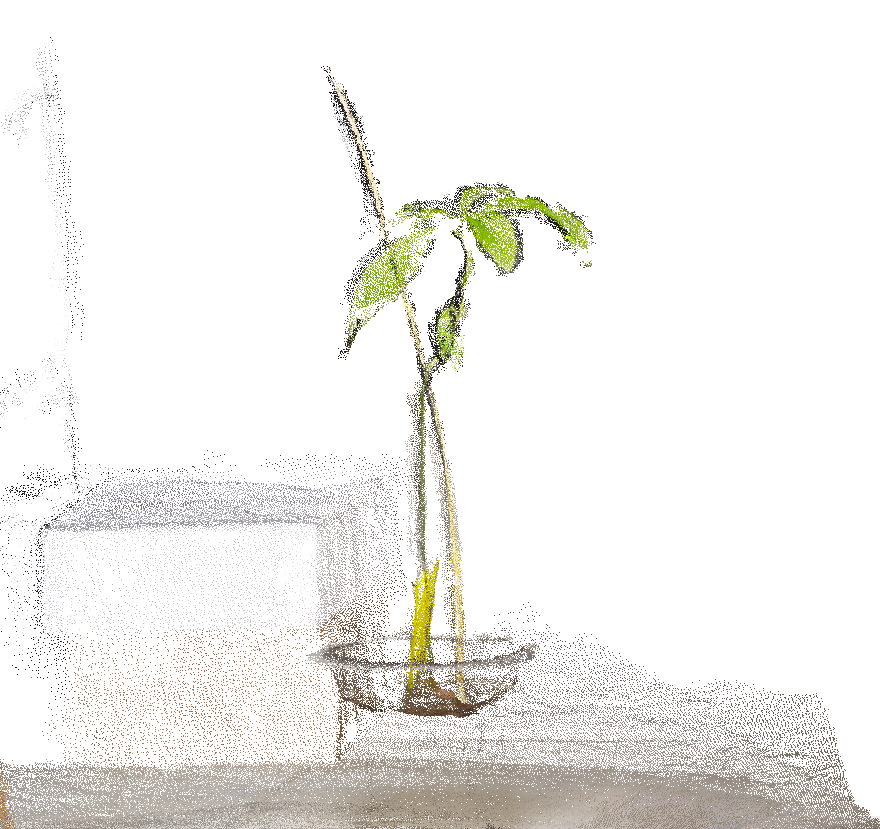
\includegraphics[width=1.0\textwidth]{./Images/PointCloudGeneration_odm.png}
			\caption{ODM}
			\label{fig:odm}
		\end{minipage}\hfill
		\begin{minipage}{0.475\textwidth}
			\centering
			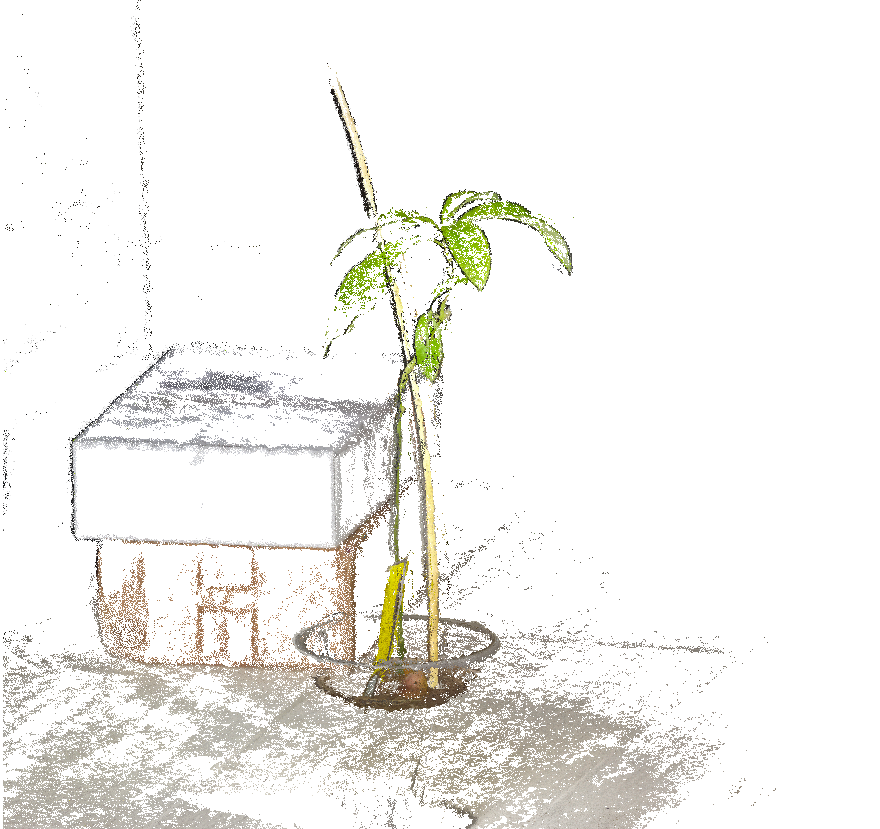
\includegraphics[width=1.0\textwidth]{./Images/PointCloudGeneration_colmap.png}
			\caption{Colmap}
			\label{fig:colmap}
		\end{minipage}
	\end{figure}
}
\frame{
	\frametitle{Generierung von Punktwolken} 
	\begin{figure}
		\centering
		\begin{minipage}{0.3\textwidth}
			\centering
			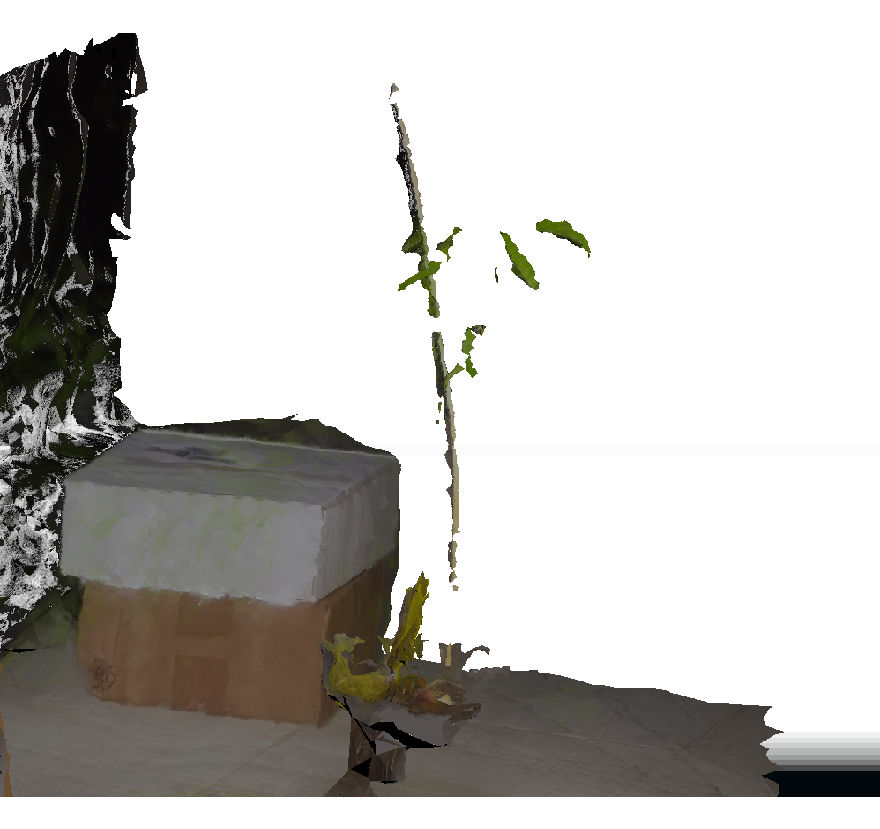
\includegraphics[width=1.0\textwidth]{./Images/PointCloudGeneration_meshroom.png}
			\caption{Meshroom}
			\label{fig:meshroom}
		\end{minipage}\hfill
		\begin{minipage}{0.3\textwidth}
			\centering
			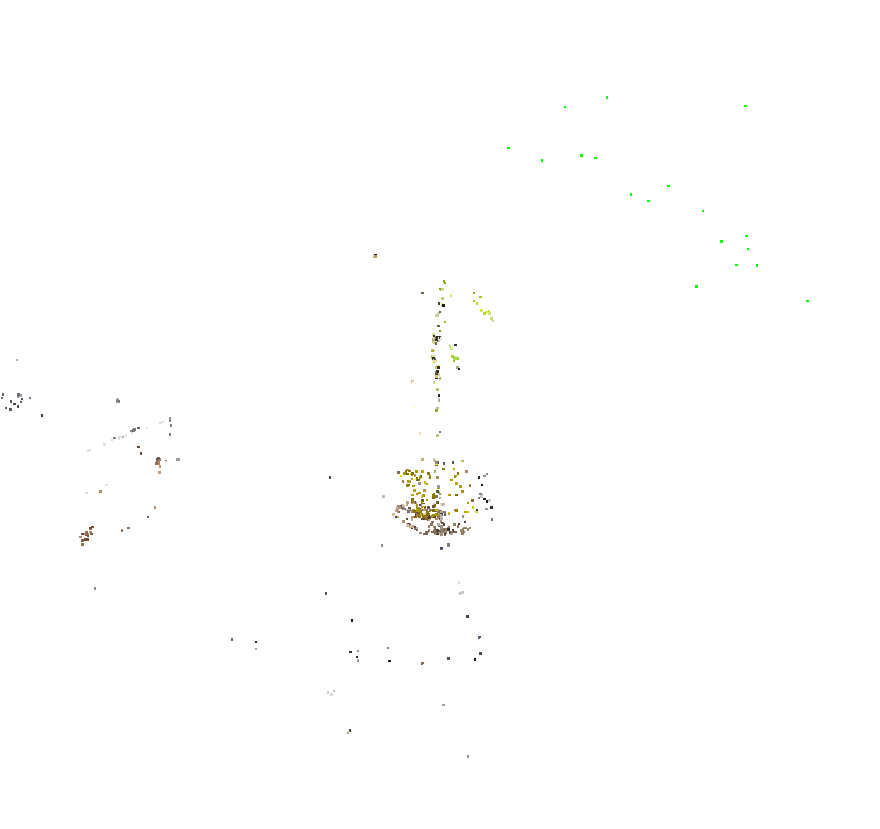
\includegraphics[width=1.0\textwidth]{./Images/PointCloudGeneration_openmvg.png}
			\caption{OpenMVG}
			\label{fig:openmvg}
		\end{minipage}\hfill
		\begin{minipage}{0.3\textwidth}
			\centering
			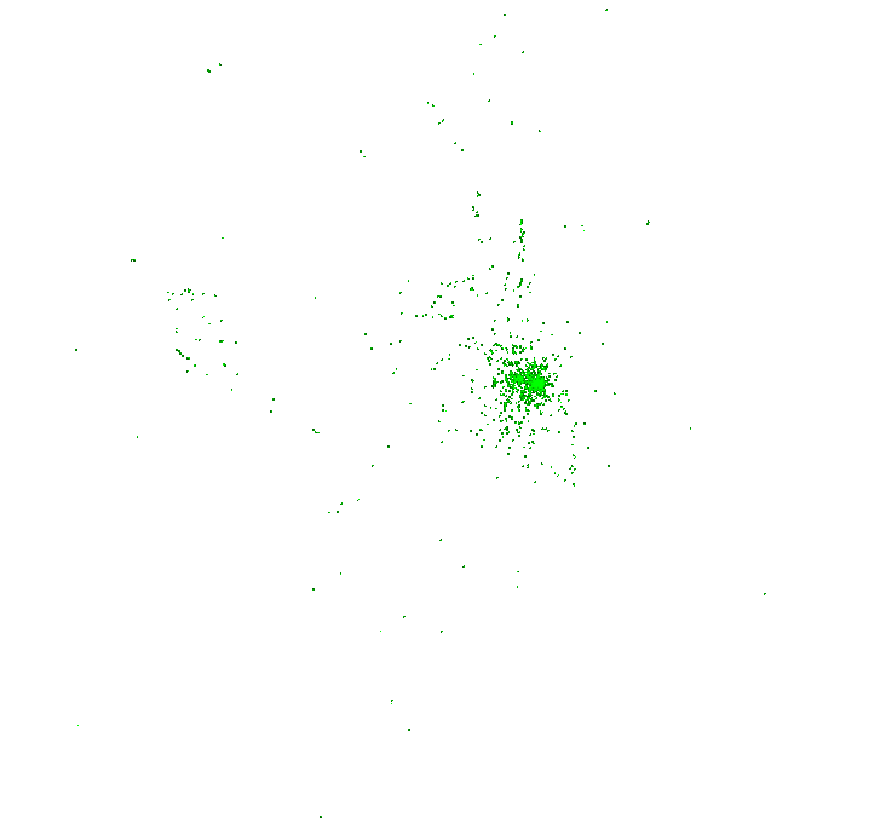
\includegraphics[width=1.0\textwidth]{./Images/PointCloudGeneration_opencv.png}
			\caption{OpenCV}
			\label{fig:opencv}
		\end{minipage}
	\end{figure}
}

\section{Segmentierung}
\frame{
	\frametitle{Segmentierung - Pflanze} 
	\begin{itemize}
		\item Ansatz 1: Entscheidung auf Basis der Krümmung eines Punktes
		\item Je höher die Krümmung eines Punktes ist, desto wahrscheinlicher gehört dieser zu einem Stiel.
		\begin{equation}
			\label{eq:manuell_classifier}
			f(p_i) = \left\{
			\begin{array}{ll}
			1 & k(p_i) \geq T_k \\
			0 & \, \textrm{sonst} \\
			\end{array}
			\right. 
		\end{equation}
		\item Problem: Es muss eine gute Parametrisierung für alle Pflanzen-Arten gefunden werden.
		\item Problem: Blätter haben teilweise ähnliche Krümmung wie Stiele.
		\item Nachteil: Entfernung des Hintergrundes bleibt offen.
		\item Nachteil: Es liegt lediglich ein binärer Classifier vor. Es können nur die Stiele von dem Rest der Pflanze differenziert werden.
		\item Nachteil: Es müssen Normalen bekannt sein.
	\end{itemize}
}
\frame{
	\frametitle{Segmentierung - Pflanze} 
	\begin{figure}
		\centering
		\begin{minipage}{0.475\textwidth}
			\centering
			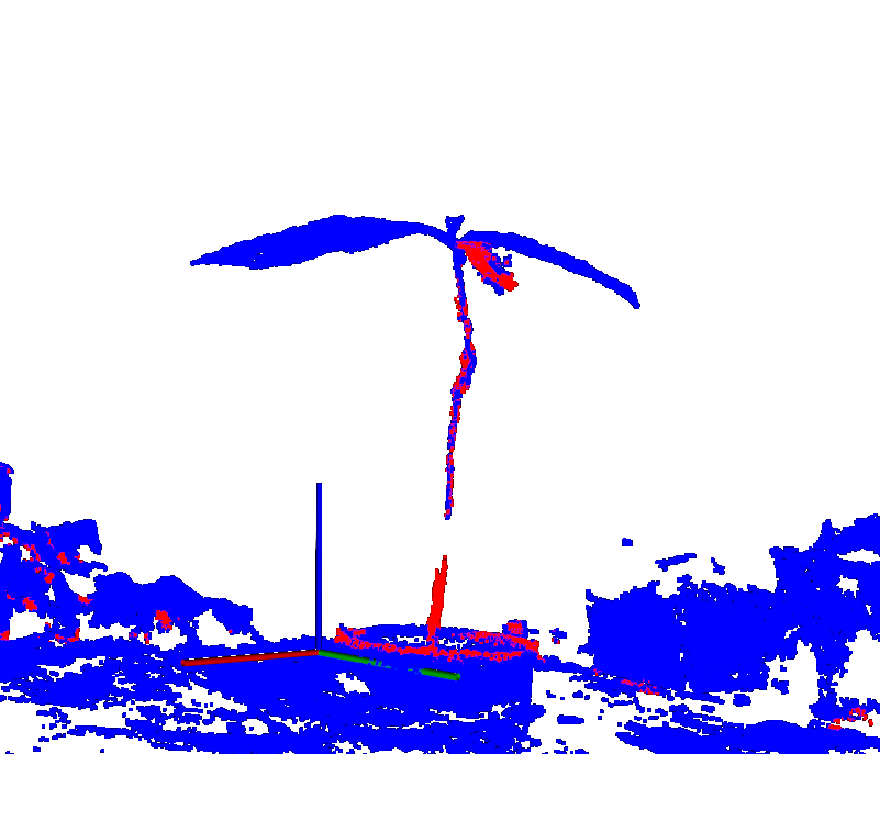
\includegraphics[width=1.0\textwidth]{./Images/HandcraftedClassifierAvocado.png}
			\caption{Avocado Ansatz 1}
			\label{fig:classifier:1:1}
		\end{minipage}\hfill
		\begin{minipage}{0.475\textwidth}
			\centering
			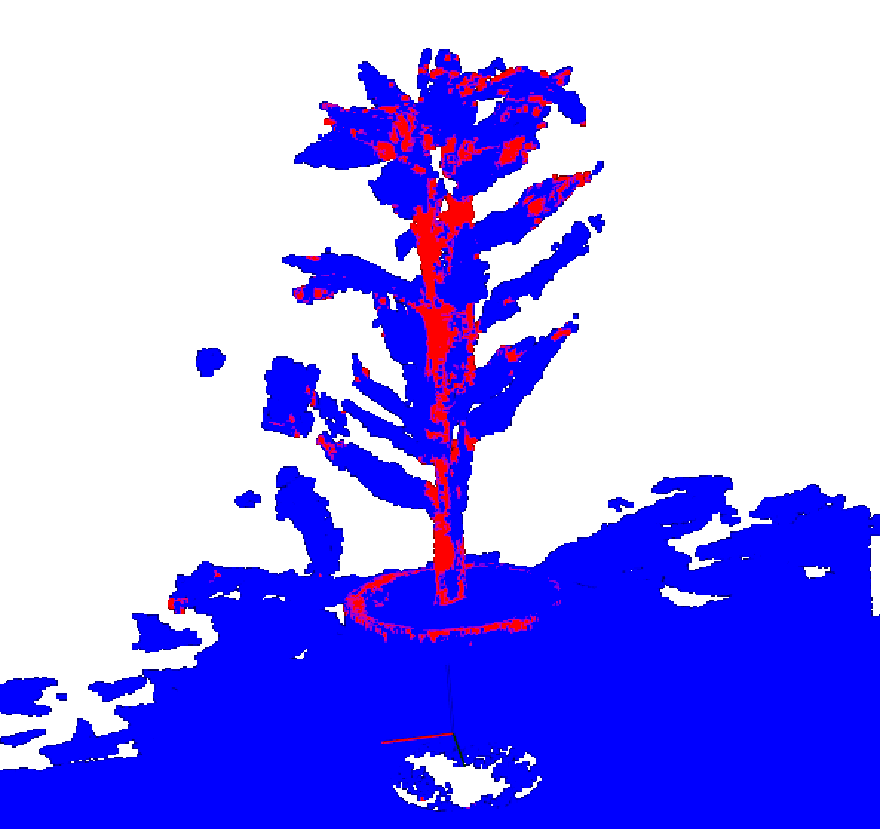
\includegraphics[width=1.0\textwidth]{./Images/HandcraftedClassifierPlant2.png}
			\caption{Zimmerpflanze Ansatz 1}
			\label{fig:classifier:1:2}
		\end{minipage}
	\end{figure}
}
\frame{
	\frametitle{Segmentierung - Pflanze} 
	\begin{itemize}
		\item Ansatz 2: Nutzung von Neuronalen Netzen (PointNet++ \cite{qi2017pointnet++})
		\item Erstellen eines Trainings-Datensatzes aus 144 individuellen Punktwolken, mit bis zu 20 Subsamples je Punktwolke.
		\item Nutzung des Datensatzes in verschiedenen Trainings-Szenarien.
		\begin{itemize}
			\item Mit und ohne Hintergrund
			\item Hintergrund mit und ohne Zentrum
			\item Mit und ohne Normalen
			\item Mit und ohne Normalisierung
			\item Mit und ohne zufällige Rotationen
		\end{itemize}
		\item Vorteil: Neben Stielen können weitere Klassen segmentiert werden. 
		\item Nachteil: Erstellen der Trainings-Daten sehr Zeit aufwendig + Daten müssen verfügbar sein.
	\end{itemize}
}
\frame{
	\frametitle{Segmentierung - Pflanze} 
	\begin{figure}
		\centering
		\begin{minipage}{0.475\textwidth}
			\centering
			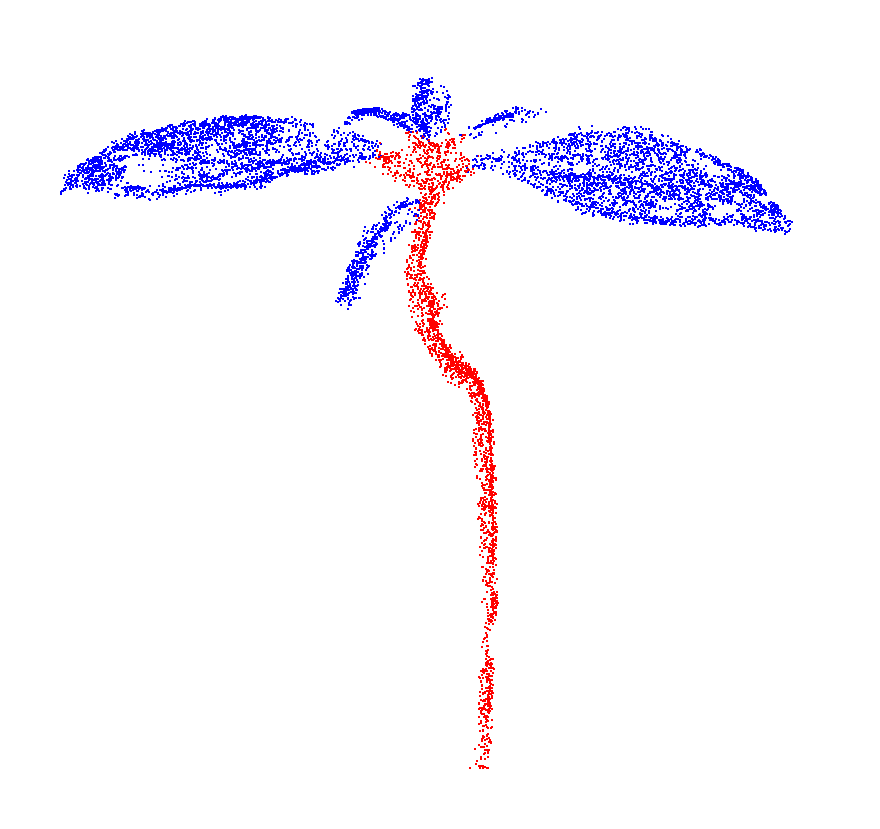
\includegraphics[width=1.0\textwidth]{./Images/Plant_Avocado.png}
			\caption{Avocado Ansatz 2}
			\label{fig:classifier:2:1}
		\end{minipage}\hfill
		\begin{minipage}{0.475\textwidth}
			\centering
			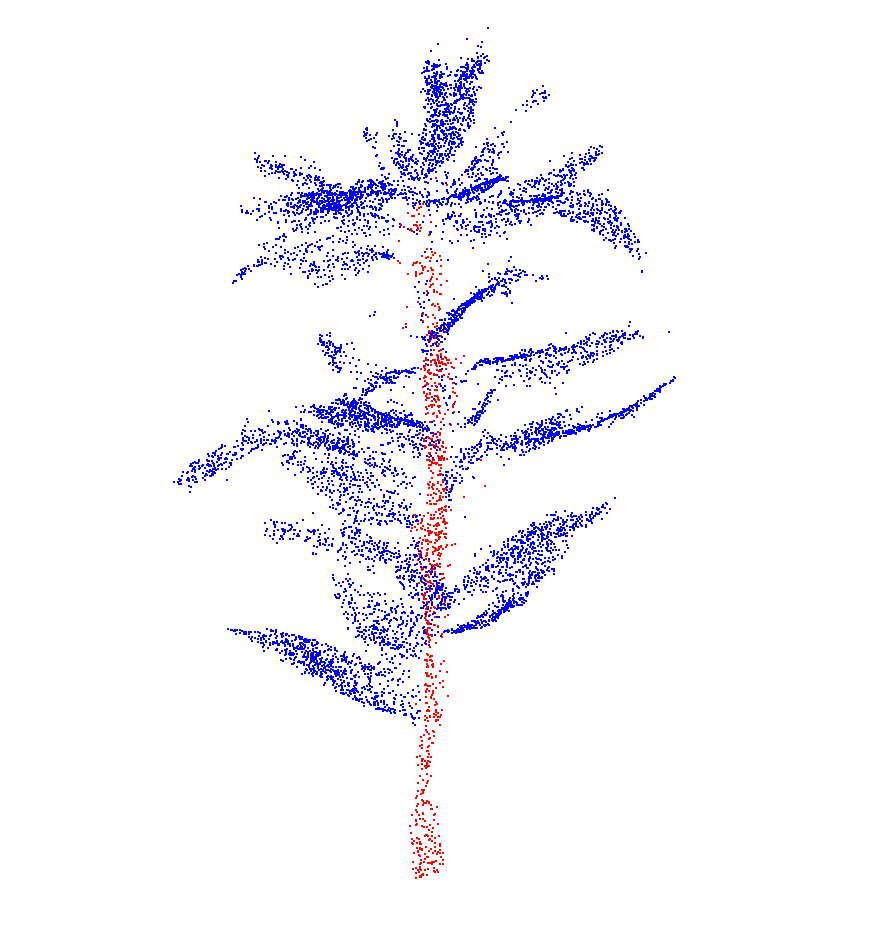
\includegraphics[width=1.0\textwidth]{./Images/Plant_Plant2.png}
			\caption{Zimmerpflanze Ansatz 2}
			\label{fig:classifier:2:2}
		\end{minipage}
	\end{figure}
}
\frame{
	\frametitle{Segmentierung - Hintergrund} 
	\begin{itemize}
		\item Auch hier wurde PointNet++ verwendet.
		\item Problem: Ergebnisse der Hintergrundsegmentierung sind durch den großen Anteil der Hintergrund-Punkte teilweise fehlerhaft.
		\item Lösung: Nur Bereich um das Zentrum der Punktwolke betrachten und Nachbearbeitung des Segmentierungs-Ergebnisses.
		\item Problem: Pflanzen, die ungewollt mit in der Szene enthalten sind, werden mit in die Analyse aufgenommen.
		\item Potentielle Lösung: Szenen-Analyse
		\begin{itemize}
			\item Einzelne Pflanzen sollen in der Szene erkannt werden.
			\item Isolieren der einzelnen Pflanzen
			\item Wenn nötig Hintergrund-Segmentierung
			\item Pflanze klassifizieren um Unkräuter auszublenden
			\item Segmentierung einzelner Pflanzen
		\end{itemize}
		%\item Lösung: Hier besser eine Szenen-Analyse durchführen und auf Bereichen die als Pflanze erkannt wurden Hintergrund-Segmentierung anwenden um Pflanze freizustellen.
	\end{itemize}
}
\frame{
	\frametitle{Segmentierung - Hintergrund} 
	\begin{figure}
		\centering
		\begin{minipage}{0.475\textwidth}
			\centering
			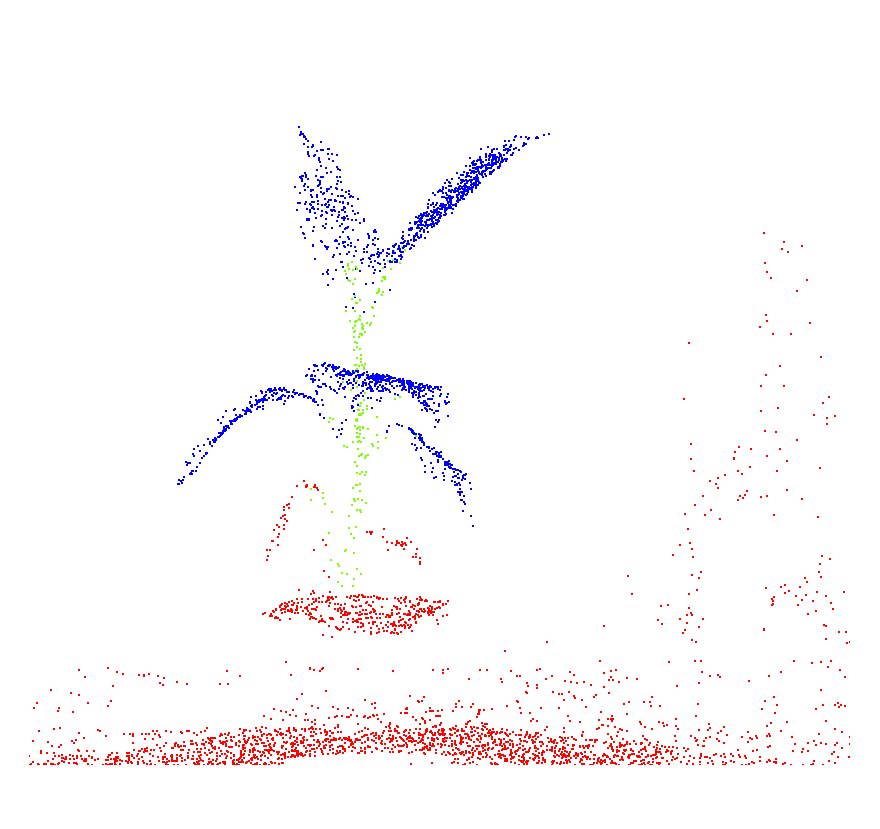
\includegraphics[width=1.0\textwidth]{./Images/BG_Banana.png}
			\caption{Hintergrundsegmentierung Bananenpflanze }
			\label{fig:segmentation:background:banana}
		\end{minipage}\hfill
		\begin{minipage}{0.475\textwidth}
			\centering
			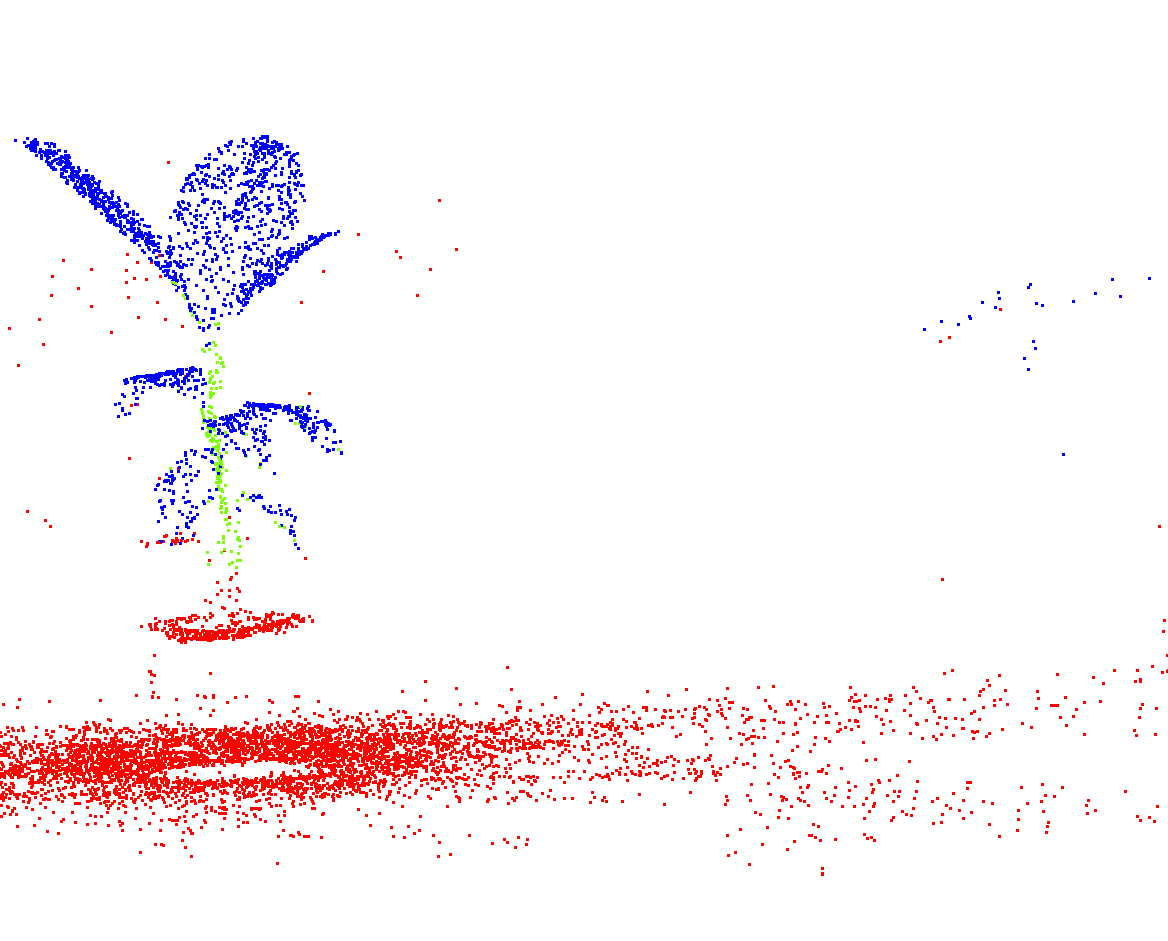
\includegraphics[width=1.0\textwidth]{./Images/BackgroundSegmentationError.png}
			\caption{Avocado-Pflanze in Szene}
			\label{fig:segmentation:background:banana:avocado}
		\end{minipage}
	\end{figure}
}
\frame{
	\frametitle{Segmentierung - Training 1} 
	\begin{figure}
		\centering
		\begin{minipage}{0.475\textwidth}
			\centering
			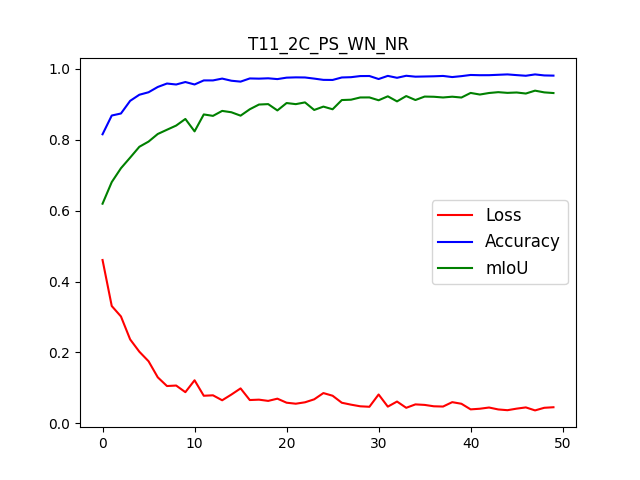
\includegraphics[width=1.0\textwidth]{./Images/T11_2C_PS_WN_NR.png}
			\caption{Ohne Hintergrund}
			\label{fig:segmentation:eval:no:background}
		\end{minipage}\hfill
		\begin{minipage}{0.475\textwidth}
			\centering
			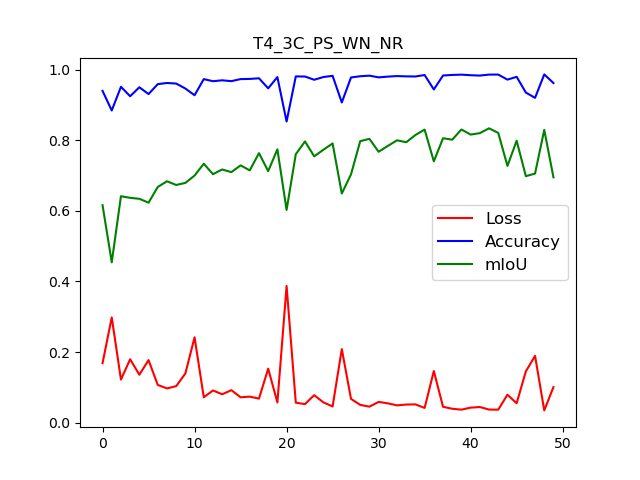
\includegraphics[width=1.0\textwidth]{./Images/T4_3C_PS_WN_NR.png}
			\caption{Mit Hintergrund}
			\label{fig:segmentation:eval:background}
		\end{minipage}
	\end{figure}
}
\frame{
	\frametitle{Segmentierung - Training 2} 
	\begin{figure}
		\centering
		\begin{minipage}{0.475\textwidth}
			\centering
			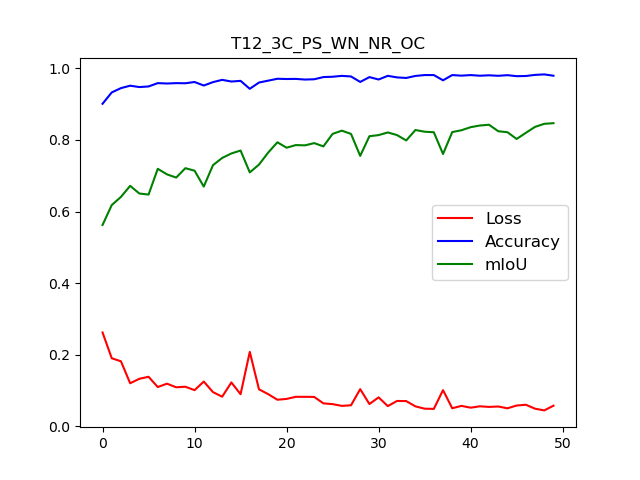
\includegraphics[width=1.0\textwidth]{./Images/T12_3C_PS_WN_NR_OC.png}
			\caption{Hintergrund nur Zentrum}
			\label{fig:segmentation:eval:center:background}
		\end{minipage}\hfill
		\begin{minipage}{0.475\textwidth}
			\centering
			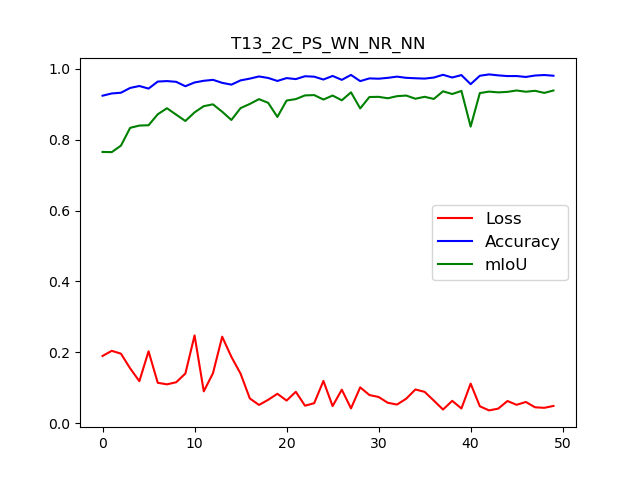
\includegraphics[width=1.0\textwidth]{./Images/T13_2C_PS_WN_NR_NN.png}
			\caption{Ohne Normalen}
			\label{fig:segmentation:eval:background}
		\end{minipage}
	\end{figure}
}
\frame{
	\frametitle{Segmentierung - Training 3} 
	\begin{figure}
		\centering
		\begin{minipage}{0.475\textwidth}
			\centering
			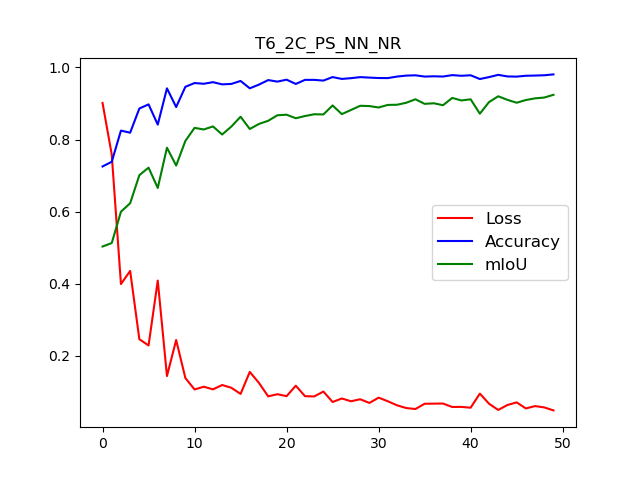
\includegraphics[width=1.0\textwidth]{./Images/T6_2C_PS_NN_NR.png}
			\caption{Ohne Normalisierung ohne Hintergrund}
			\label{fig:segmentation:eval:not:normalized}
		\end{minipage}\hfill
		\begin{minipage}{0.475\textwidth}
			\centering
			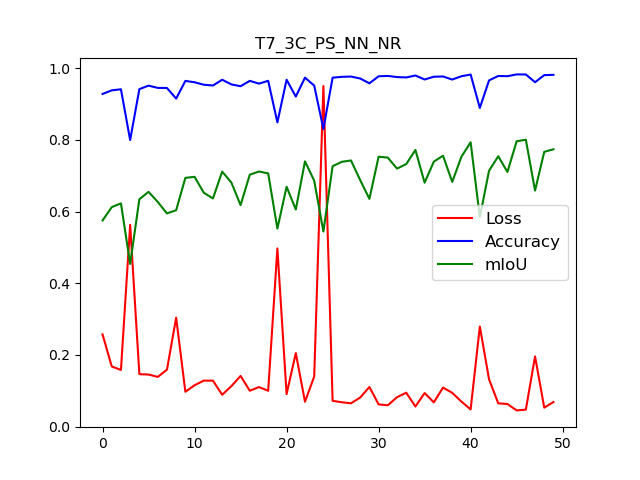
\includegraphics[width=1.0\textwidth]{./Images/T7_3C_PS_NN_NR.png}
			\caption{Ohne Normalisierung mit Hintergrund}
			\label{fig:segmentation:eval:not:normalized:background}
		\end{minipage}
	\end{figure}
}
\frame{
	\frametitle{Segmentierung - Training 4} 
	\begin{figure}
		\centering
		\begin{minipage}{0.475\textwidth}
			\centering
			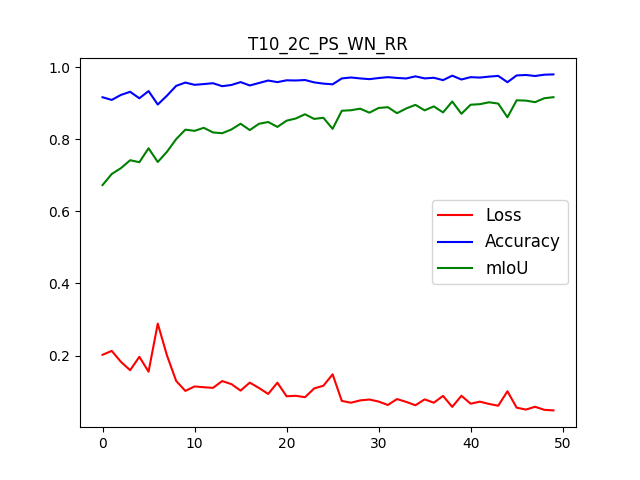
\includegraphics[width=1.0\textwidth]{./Images/10_2C_PS_WN_RR.png}
			\caption{Mit zufälliger Rotation ohne Hintergrund}
			\label{fig:segmentation:eval:random:rotation}
		\end{minipage}\hfill
		\begin{minipage}{0.475\textwidth}
			\centering
			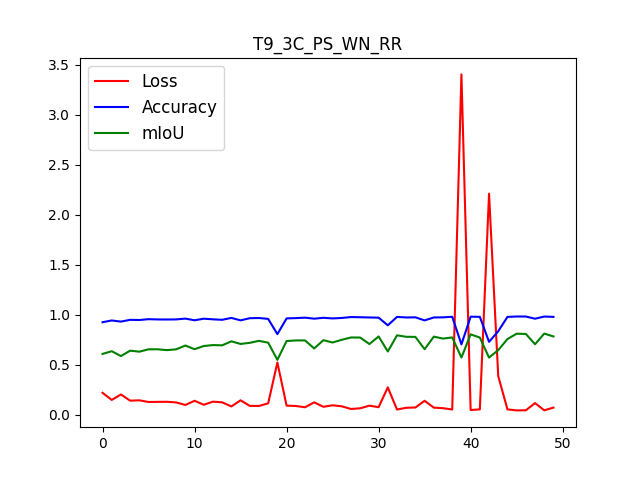
\includegraphics[width=1.0\textwidth]{./Images/9_3C_PS_WN_RR.png}
			\caption{Mit zufälliger Rotation mit Hintergrund}
			\label{fig:segmentation:eval:random:rotation:background}
		\end{minipage}
	\end{figure}
}
\frame{
	\frametitle{Segmentierung - Evaluation} 
	\begin{table}
		\begin{center}
		\resizebox{\linewidth}{!}{
		\begin{tabular}{|l || c | c | c | c || c | c | c | c |} 
			\hline
			 & \thead{t11}  & \thead{t6} & \thead{t10} & \thead{t13} & \thead{t4} & \thead{t7} & \thead{t12} & \thead{t9}  \\  
			\hline
			\hline
			Loss & $0,044$ & $0,056$& $0,079$& $0,127$& $0,038$& $0,054$& $0,051$& $0,05$\\
			\hline
			Genauigkeit & $0,98$& $0,976$& $0,969$& $0,95$& $0,986$& $0,981$& $0,98$& $0,982$\\
			\hline
			mIoU & $0,925$& $0,908$& $0,893$& $0,827$& $0,813$& $0,788$& $0,841$& $0,811$\\
			\hline
		\end{tabular}}
		\end{center}
		\caption{Evaluations-Ergebnisse der verschiedenen Modelle. Links ohne Hintergrund (t11, t6, t10, t13). Rechts mit Hintergrund (t9, t4, t7, t12).}
		\label{tab:segmentation:eval}
	\end{table}
}
\section{Registrierung}
\frame{
	\frametitle{Registrierung} 
	\begin{itemize}
		\item Problem: Da beim Erstellen der Punktwolke mit SfM der Maßstab nicht ermittelt werden kann, liegen verschiedene Punktwolken derselben Szene in unterschiedlichen Maßstäben vor.
		\item Lösung: Punktwolken mit einer Hintergrund-Punktwolke registrieren, um alle Punktwolken einer Messreihe im selben Maßstab vorliegen zu haben.
		\begin{equation}
			\label{eq:icp}
			\underset{R,t}{\operatorname{argmin}}(\sum_{i=1}^N{\|Rp_{s_i} + t - p_{t_i}\|^2})
		\end{equation}
		\item Problem: Die meisten Registrierungsverfahren berücksichtigen nicht die Skalierung.
		\begin{equation}
			\label{eq:icp}
			\underset{R,t,s}{\operatorname{argmin}}(\sum_{i=1}^N{\|R(sp_{s_i}) + t - p_{t_i}\|^2})
		\end{equation}
		\item Es wurden mehrere Ansätze untersucht dieses Problem zu lösen.
	\end{itemize}
}
\frame{
	\frametitle{Registrierung - ICP mit Schätzung der Skalierung} 
	\begin{itemize}
		\item In der Bibliothek Point Cloud Libary (PCL) wird eine Implementation, die auch einen Wert für die Skalierung liefert, bereit gestellt.
		\item Problem: ICP benötigt gute Initialisierung.
		\item Initialisierung finden:
		\begin{itemize}
			\item Punktwolken an der XY-Ebene ausrichten.
			\item Bereich um Zentrum entnehmen.
			\item Punktwolken auf dieselbe Größe bringen.
			\item Störung herausfiltern.
			\item Initiale Registrierung mit ausgewählten Punkten.
		\end{itemize}
		\item Nach Schätzung der Skalierung folgt abschließende Registrierung.
		\item Problem: Ansatz funktioniert nur bedingt für einige Punktwolken.
	\end{itemize}
}
\frame{
	\frametitle{Registrierung - DCP anpassen} 
	\begin{itemize}
		\item Deep Closest Points (DCP)\cite{Wang_2019_ICCV} ist ein Neuronales Netz, welches das Registrierungsproblem löst, aber keine Schätzung der Skalierung liefert.
		\item SVD-Head anpassen und Eingabe mit Einsen erweitern.
		\item Resultat der SVD ist nun eine $4 \times 4$ Matrix.
		\item Die Annahme, dass diese Matrix als Transformations-Matrix interpretiert werden kann, hat sich nicht bestätigt.
		\item Besser: Berechnung der Skalierung auf Basis der Rotation wie in \cite{Ziner2005PointSR}.
		%\begin{equation}
		%	\label{eq:icp_scale:1}
		%	s_i = R (p_{s_i} - \bar{p_s}),\quad t_j = p_{t_j} - \bar{p_t}
		%\end{equation}
		%\begin{equation}
		%	\label{eq:icp_scale:2}
		%	\hat{s} = \sum_{i,j}{t_j^Ts_i} / \sum_{i}{s_i^Ts_i}
		%\end{equation}
		%\begin{equation}
		%	\label{eq:icp_scale:3}
		%	t = \bar{p_t} - \hat{s}  R \bar{p_s}
		%\end{equation}
	\end{itemize}
}
\frame{
	\frametitle{Registrierung - Iterative Schätzung der Skalierung} 
	\begin{itemize}
		\item Iteratives durchlaufen verschiedener Skalierungen mit anschließender Registrierung.
		\item Wahl der besten Iteration durch Messen des Abstands zwischen den Punktwolken oder Nutzung des Fehlermaßes der einzelnen Implementationen.
		\item Einsatz von verschiedenen Registrierungsverfahren möglich. 
		\begin{itemize}
			\item PointNetLK \cite{aoki2019pointnetlk}
			\item DCP \cite{Wang_2019_ICCV}
			\item RPM-Net \cite{Yew_2020}
			\item ICP (open3d) \cite{zhou2018open3d}
			\item RICP \cite{ICP}
		\end{itemize}
		\item RPM-Net und ICP haben sich hier als robust erwiesen.
		\item Relativ gute Ergebnisse, aber auch hier kommt es immer wieder zu Ausreißern.
	\end{itemize}
}
\frame{
	\frametitle{Registrierung - Iterative Schätzung der Skalierung} 
	\begin{figure}
		\centering
		\begin{minipage}{0.3\textwidth}
			\centering
			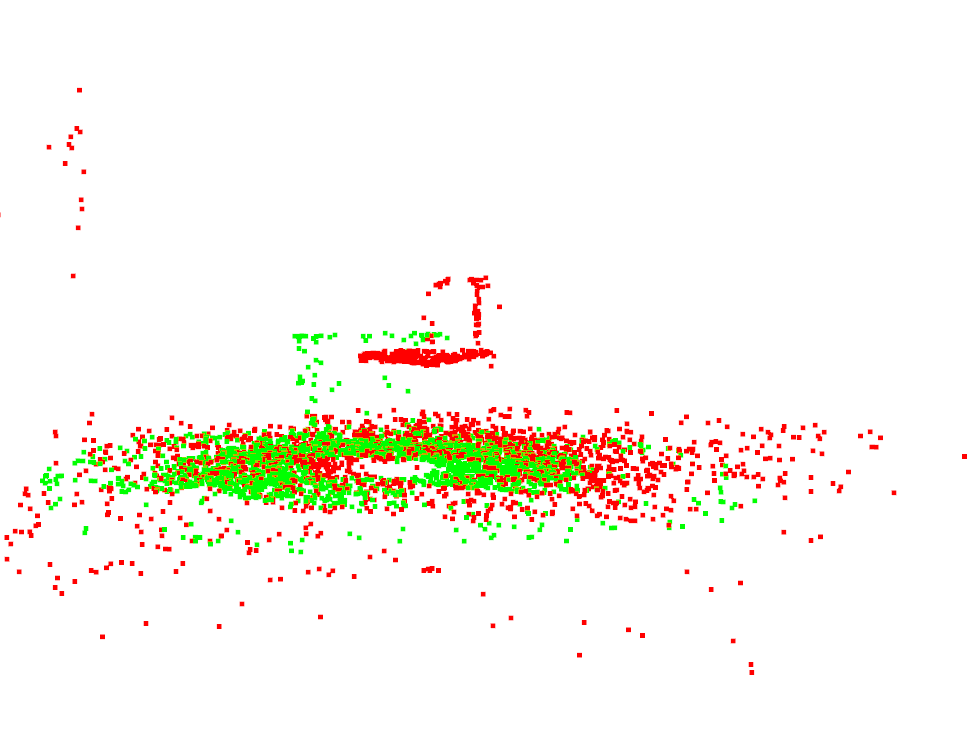
\includegraphics[width=1.0\textwidth]{./Images/RegistrationBananaT1.png}
			\label{fig:reg:t1}
		\end{minipage}\hfill
		\begin{minipage}{0.3\textwidth}
			\centering
			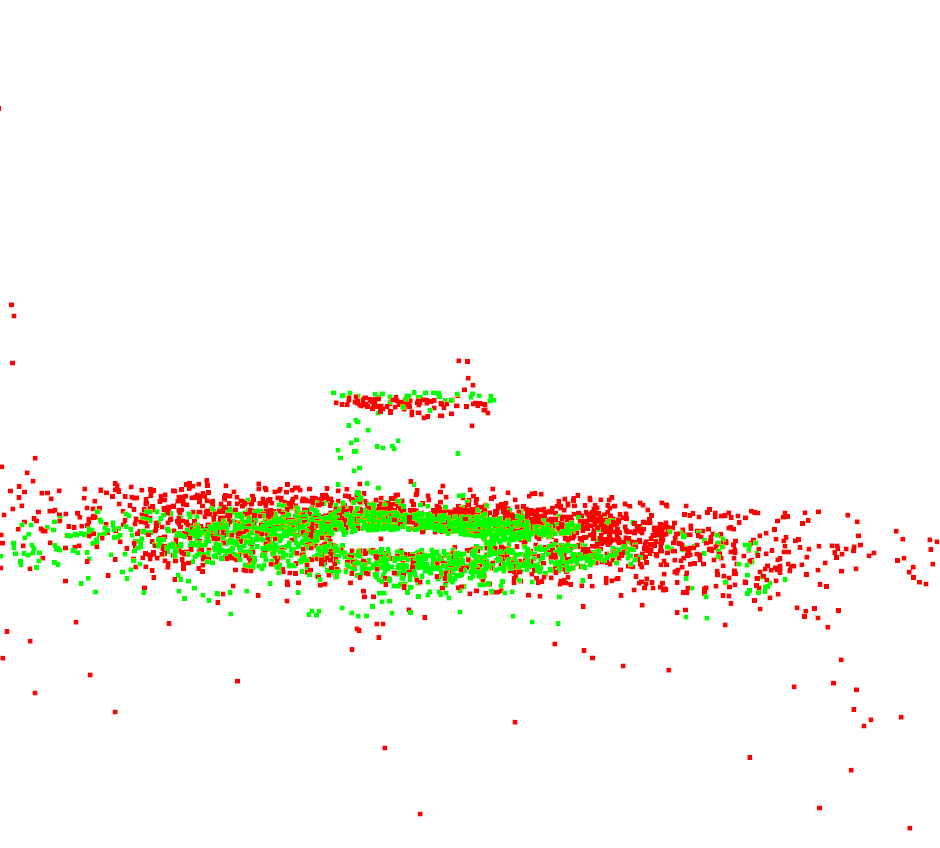
\includegraphics[width=1.0\textwidth]{./Images/RegistrationBananaT2.png}
			\label{fig:reg:t2}
		\end{minipage}\hfill
		\begin{minipage}{0.3\textwidth}
			\centering
			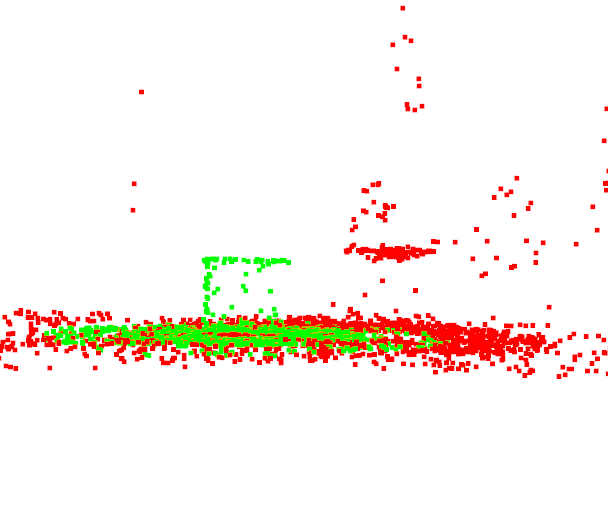
\includegraphics[width=1.0\textwidth]{./Images/RegistrationBananaT3.png}
			\label{fig:reg:t3}
		\end{minipage}
		\caption{Registrierungsergebnisse für drei Zeitpunkte einer Pflanze}
	\end{figure}
}
\frame{
	\frametitle{Registrierung - Iterative Schätzung der Skalierung} 
	\begin{figure}
		\centering
		\begin{minipage}{0.475\textwidth}
			\centering
			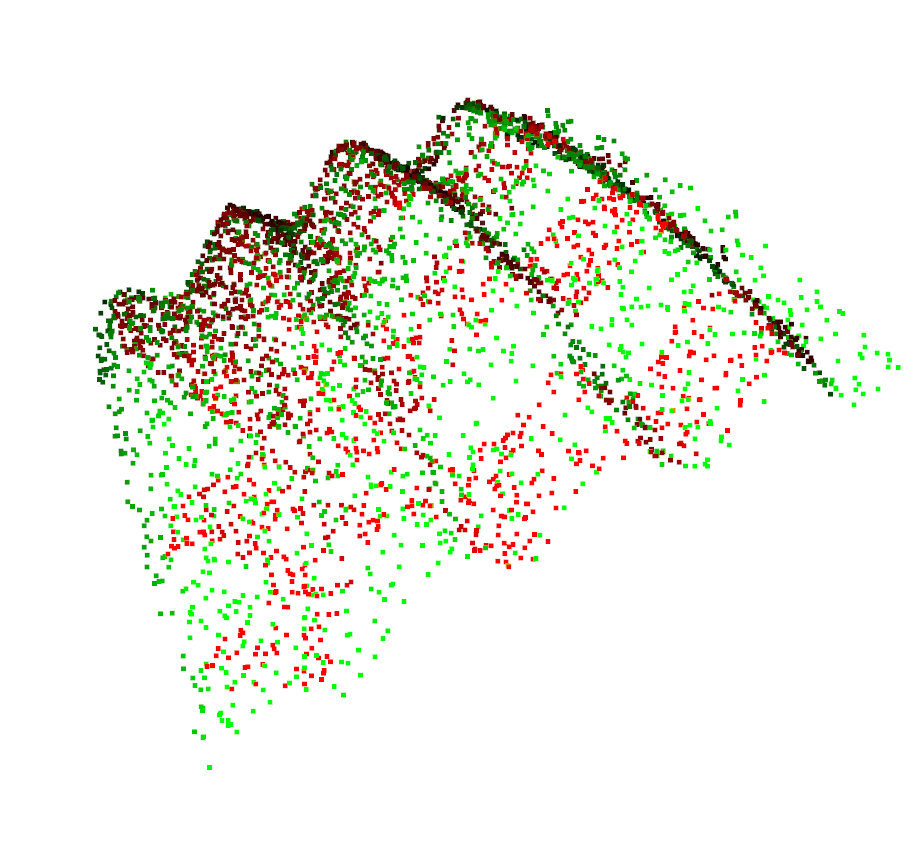
\includegraphics[width=1.0\textwidth]{./Images/Registration_Sinus.png}
			\label{fig:generated:surface:sinus}
		\end{minipage}\hfill
		\begin{minipage}{0.475\textwidth}
			\centering
			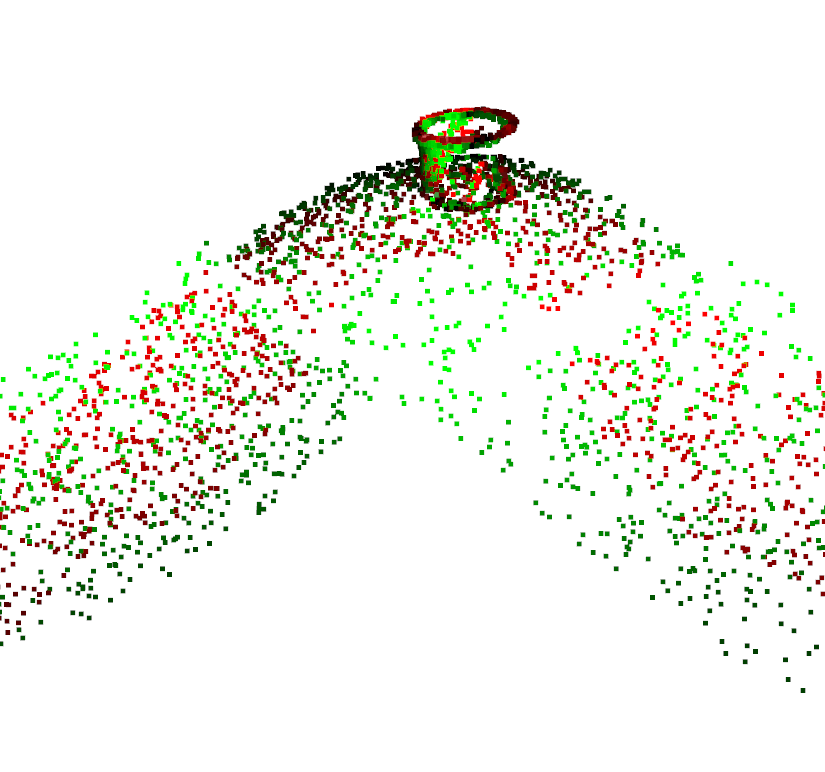
\includegraphics[width=1.0\textwidth]{./Images/Registration_Pot.png}
			\label{fig:generated:surface:pot}
		\end{minipage}
		\caption{Registrierungsergebnisse für generierte Oberflächen}
	\end{figure}
}
\frame{
	\frametitle{Segmentierung - Evaluation} 
	\begin{table}
		\begin{center}
		\resizebox{\linewidth}{!}{
			\begin{tabular}{|l || c | c | c | c | c | } 
				\hline
				 & DCP & RPM-Net & PointNetLK & ICP & RICP \\  
				\hline
				\hline
				Banane & $0,0585$ & $0,0129$& $0,1673$& $0,0117$& $0,0178$\\
				\hline
				Avocado & $0,0721$& $0,012$& $0,2235$& $0,0122$& $0,0245$\\
				\hline
			\end{tabular}
		}
		\end{center}
		\caption{Evaluations-Ergebnisse der verschiedenen Registrierungsverfahren}
		\label{tab:registration:eval}
	\end{table}
}
\section{Server}
\frame{
	\frametitle{Server - Pipelines und Jobs} 
	\begin{figure}
		\centering
		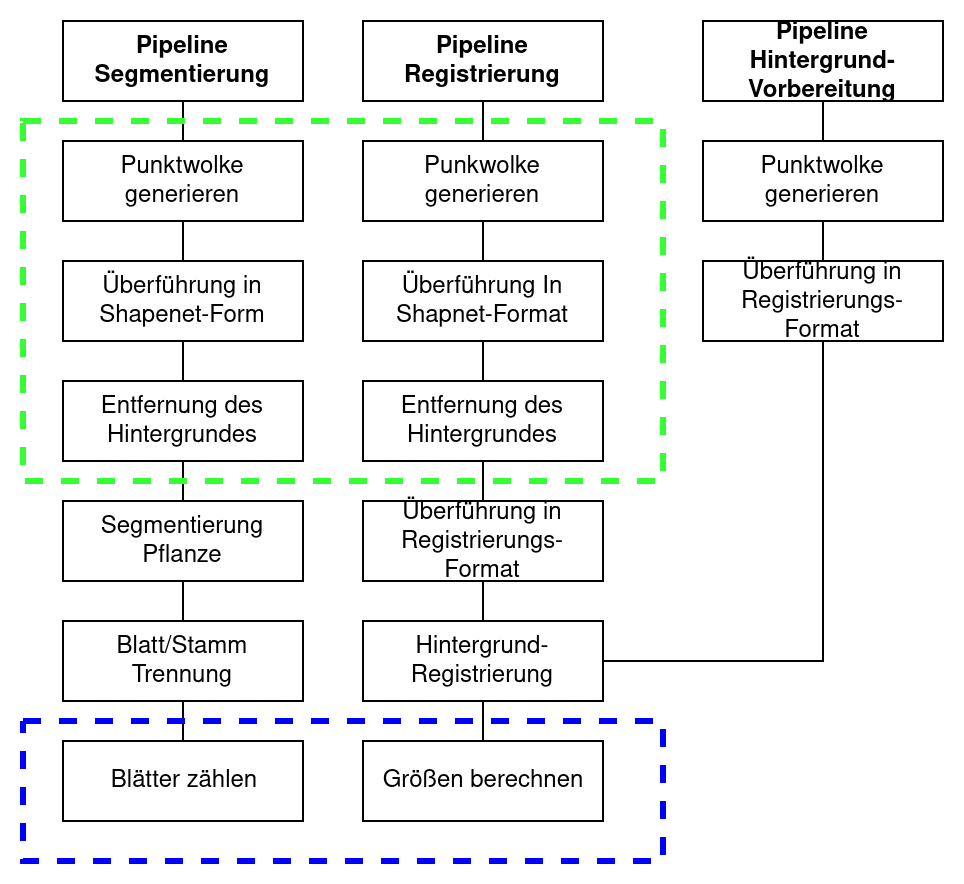
\includegraphics[width=0.65\textwidth]{./Images/Pipelines.png}
		\caption{Übersicht über die einzelnen Pipelines und die darin enthaltenen Jobs.}
		\label{fig:Pipelines}
	\end{figure}
}
\frame{
	\frametitle{Server - Schnittstelle} 
	\begin{itemize}
		\item Fünf Schnittstellen um Anwendung zu nutzen.
		\begin{itemize}
			\item POST /detail/\{Messreihe\}/\{Zeitstempel\}
			\item PUT /detail/\{Messreihe\}/\{Zeitstempel\}
			\item GET /detail/\{Messreihe\}/\{Zeitstempel\}
			\item GET /listing/\{Messreihe\}
			\item GET /result/\{Messreihe\}/\{Zeitstempel\}
		\end{itemize}
		\item Bearbeitung einzelner Jobs im Hintergrund.
		\item Zugriffe auf geteilte Ressourcen werden über Mutexe geschützt.
		\begin{itemize}
			\item Job-Queue
			\item Status
			\item Result
		\end{itemize}
	\end{itemize}
}


\section{Demo}
\frame{
	\frametitle{Demo} 
	\begin{figure}
		\centering
		\begin{minipage}{0.3\textwidth}
			\centering
			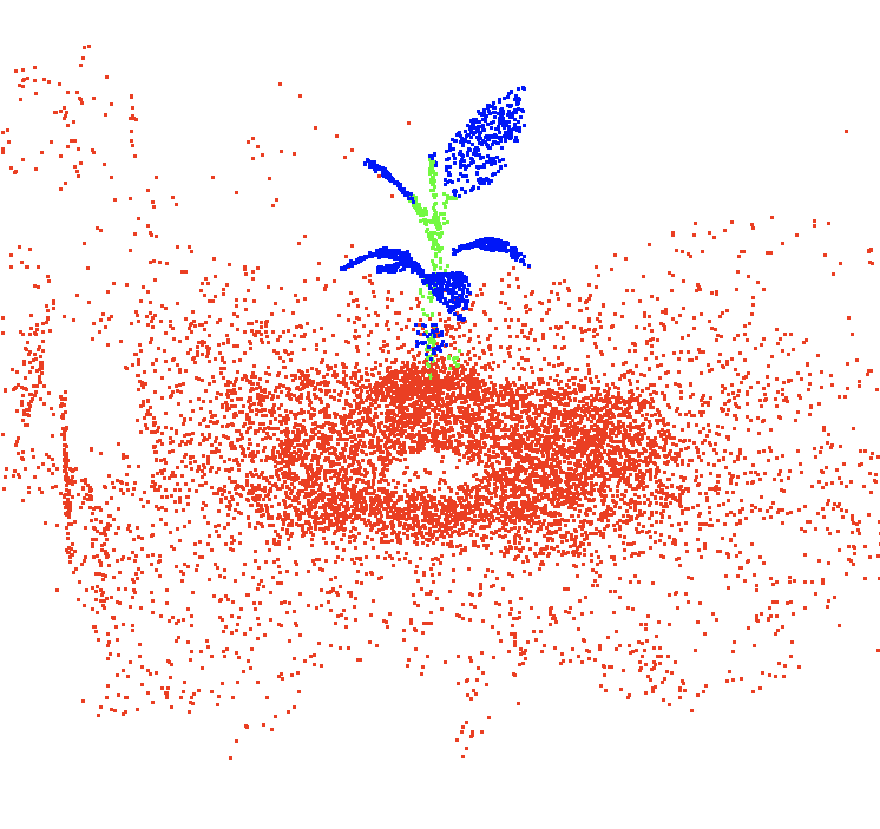
\includegraphics[height=4.5cm,width=4.5cm]{./Images/PipelineBackgroundSegmentationStriped.png}
			\caption{Hintegrund-Segmentierung}
			\label{fig:PiplineBackgroundSegmentation}
		\end{minipage}\hfill
		\begin{minipage}{0.3\textwidth}
			\centering
			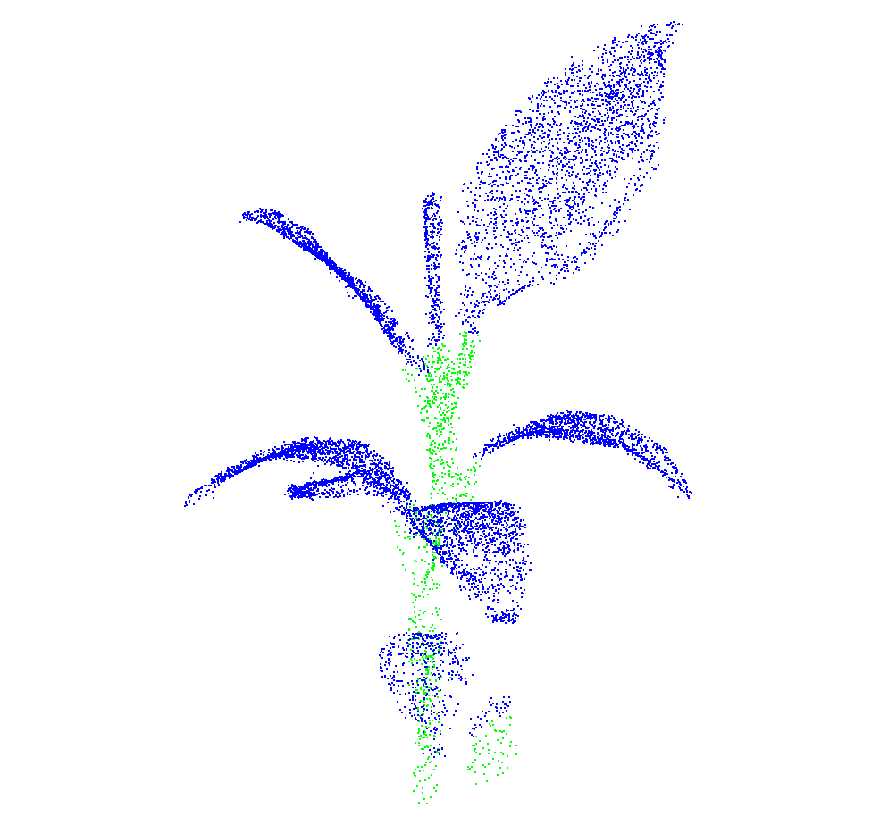
\includegraphics[height=4.5cm,width=4.5cm]{./Images/PipelinePlantSegmentation.png}
			\caption{Planzen-Segmentierung}
			\label{fig:PipelinePlantSegmentation}
		\end{minipage}\hfill
		\begin{minipage}{0.3\textwidth}
			\centering
			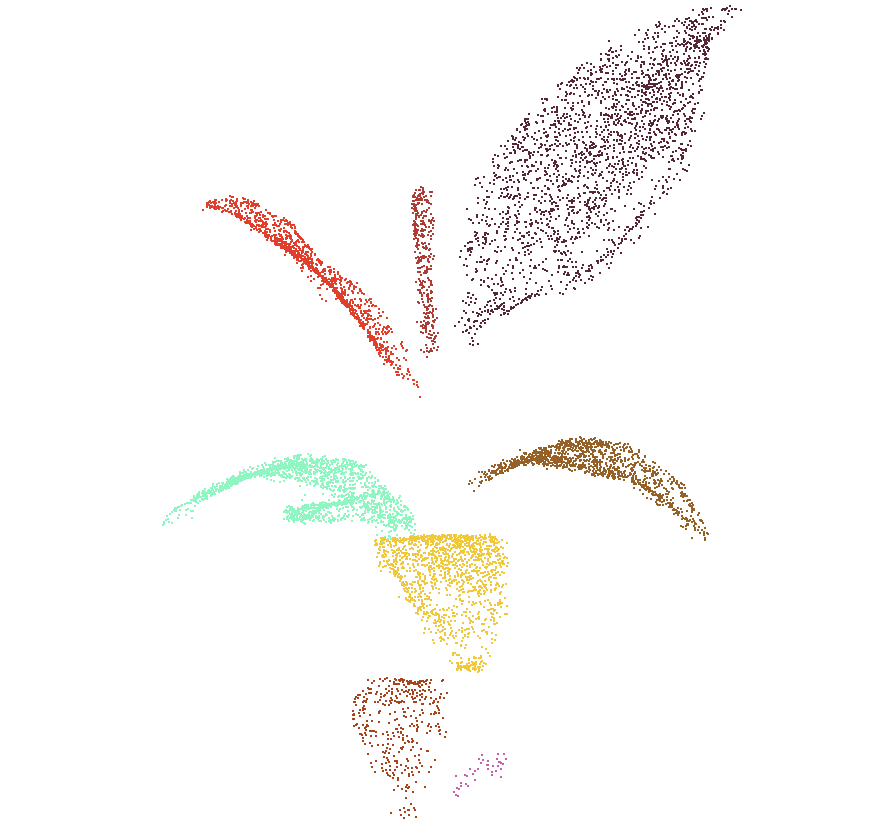
\includegraphics[height=4.5cm,width=4.5cm]{./Images/PipelineLeaveSegmentationStriped.png}
			\caption{Blatt-Segmentierung}
			\label{fig:PipelineLeaveSegmentation}
		\end{minipage}
	\end{figure}
}

\section{Quellen}
\begin{frame}[allowframebreaks]
    \frametitle{Referenzen}
    \bibliographystyle{ieeetr}
    \bibliography{./bibleografie.bib}
\end{frame}

\end{document}
